\section{Contribution}
\label{sec:contribution}

In the scope of this thesis, we developed FESDData and FESDModel, or Fault estimation for Skeleton detection for data collection and model creation. FESDData is the tool that allows us to record, analyze and it, as well as . FESD is a tool that is designed to be used by SilverFit. It is a tool that is designed to be easy to use and that can be used by anyone. 

\subsection{Developed Software}

\textit{\textbf{UNSURE} Should I write about the software, explain the OpenGL implementation, the ImGui GUI and so on?}
\textit{\textbf{TODO} Change Screenshots to light mode to be consistent with the rest of the thesis (can wait until screenshots are final)}

\begin{figure}[ht]
  \centering
  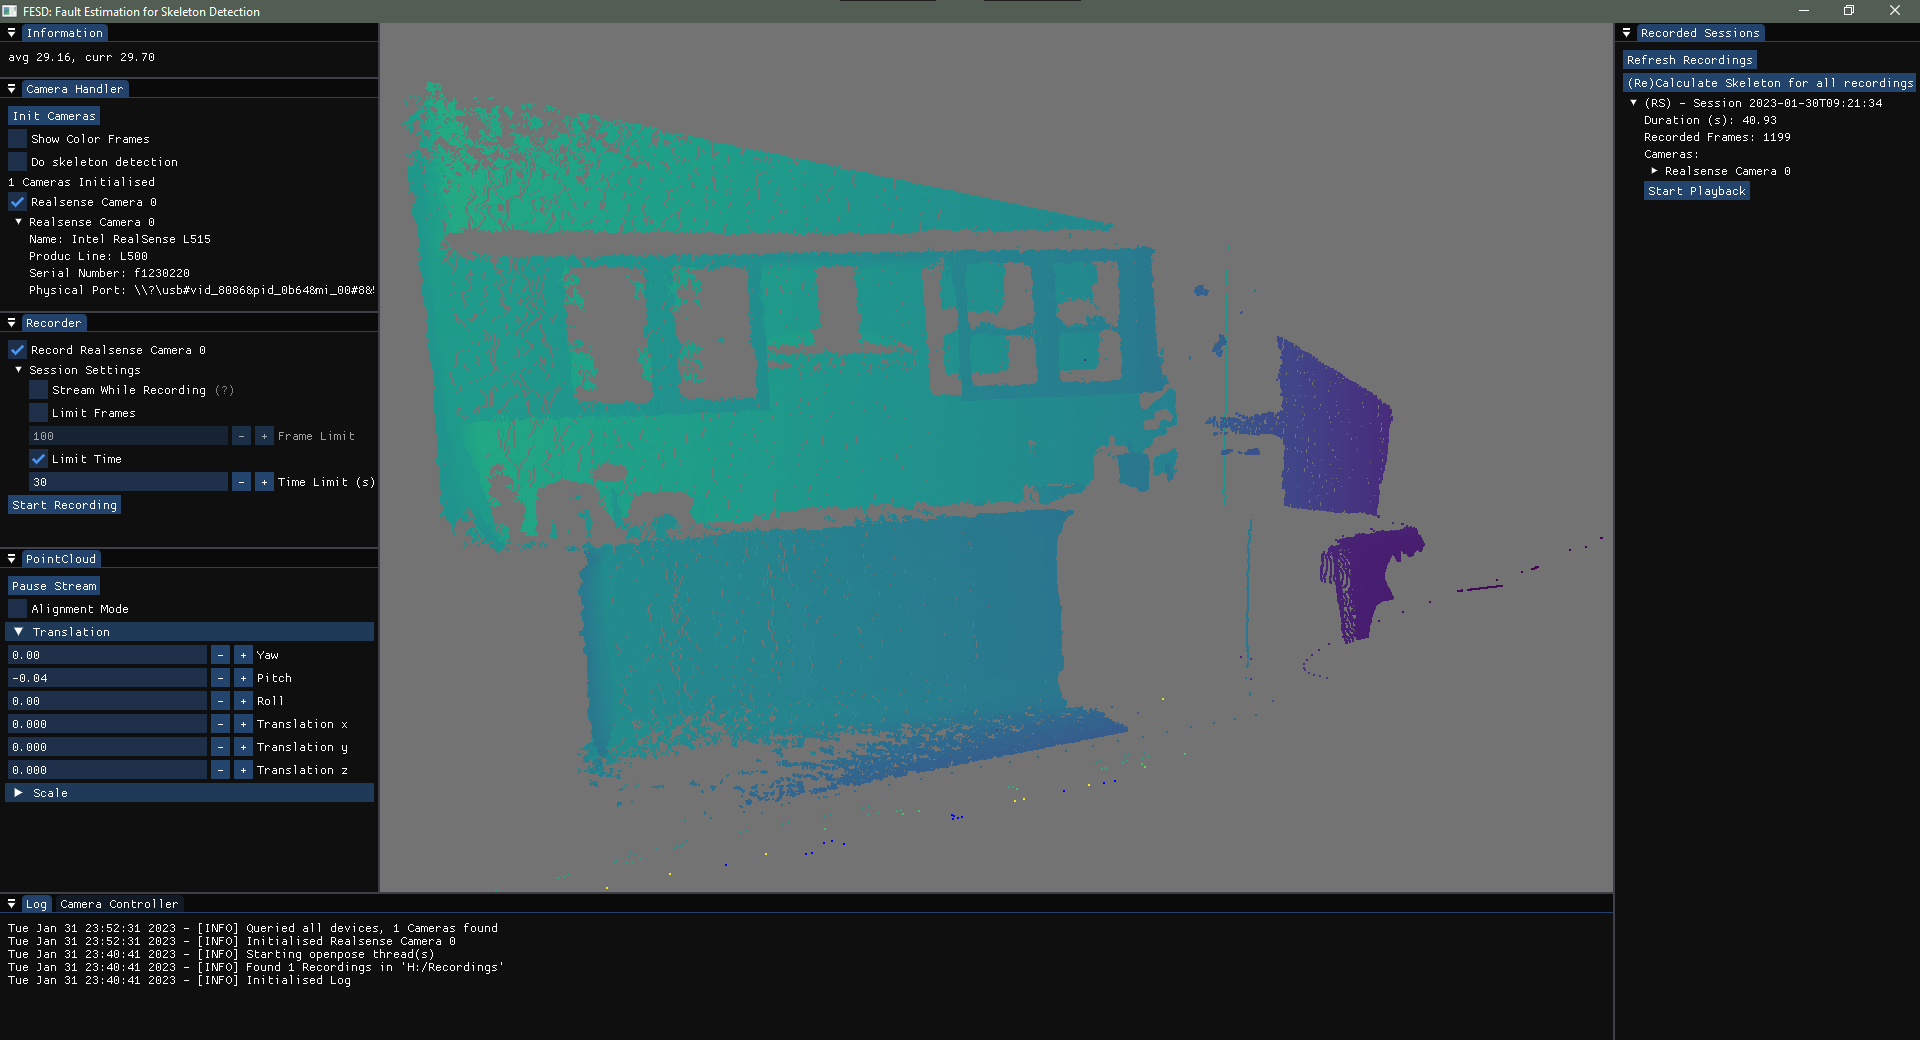
\includegraphics[width=\linewidth]{figures/FESD/all.png}
  \caption[FESD GUI]{A screenshot of the FESD GUI streaming a point cloud. The GUI is used to record and visualize the data, and to playback recordings to validate the data. The GUI is written in C++ using the ImGui framework. The Pointcloud is visualised using OpenGL and a glsl shader.}
  \label{fig:stream_gui}
\end{figure}

\subsection{Developed Model}